\chapter{Metoda 3D porównywania kodów}
Metoda opiera się na porównywaniu poprzez wykorzystanie wszystkich danych o porównaniu kodów. Decyzje o weryfikacji odcisku podejmowana jest poprzez analizę podobieństwa i niepodobieństwa jednocześnie. Do dyspozycji są 3 porównania, ale ponieważ rozkład punktów porównania 1:0 i porównania 0:1 jest prawie taki sam podjęto decyzję o pominięciu tego porównania w procesie weryfikacji. Podobnie jak w poprzednich rozdziałach sposób działania będzie porównywany z wynikami otrzymanymi od SDK $Neurotechnology$. Ten sposób porównania ma służyć nie tylko polepszeniu ogólnego wyniku algorytmu ale też i sposobu porównywania bazującego tylko na liczbie minucji dopasowanych i niedopasowanych. Niemożliwe jest jednak przedstawianie błędów w takiej samej konwencji jak w poprzednich rozdziałach. Wynika to z tego iż próg decyzyjny nie dobierany jest w taki sposób aby równoważyć błąd FAR i FRR, a poprzez tworzenie funkcji separującej zbiory punktów od siebie. Jest to o tyle kłopotliwe iż nie mam możliwości manipulowania progiem decyzyjnym tak samo jak w poprzednich rozdziałach.
Przedstawiane wyniki to wartości błędnych decyzji dopasowania i niedopasowania. Mimo iż rozpatrujemy rozkład punktów na płaszczyźnie metoda została nazwana porównaniem 3D, gdyż do weryfikacji używa trzech rodzajów porównań.
\section [Opis metody][Opis metody]{Opis metody}
Testy metody wykonano na tej samej grupie porównań co testy opierające się na badaniu podobieństwa i nie podobieństwa. Zbiór ten podzielono na dwie części, część uczącą i część testującą. Część ucząca odpowiada za utworzenie funkcji separującej oba zbiory porównań, część testująca wykorzystana jest do testów poprawnej weryfikacji dla utworzonej funkcji separującej. Testy prowadzone są w trzech wariantach
\renewcommand*{\labelitemi}{\bullet}
\begin{itemize}
	\item Rozkład porównań 1:1 do sumy porównań 1:0 i 0:1
	\item Rozkład porównań 1:1 do 1:0
	\item Rozkład porównań 1:1 do 0:1
\end{itemize}
\vspace{.5cm}\par
Dla potrzeb tej pracy wybrano metodę Maszyny wektorów nośnych\footnote{SVM z ang. support vector machine - klasyfikator, którego nauka ma na celu wyznaczenie hiperpłaszczyzny rozdzielającej z maksymalnym marginesem przykłady należące do dwóch klas.} oraz skorzystano z gotowych implementacji tej metody w środowisku MATLAB. W trakcie testów klasyfikator tworzy hiperpłaszczyzną separująca zbiory punktów, a następnie testuje wyniki dla zbioru testującego. Dopuszczalne są przypadki nie w pełni separowane. Oznacza to, że metoda ta może wnosić błąd już dla swojego zbioru uczącego. Kształt hiperpłaszczyzny zależy nie tylko od rozkładu punktów ale też od używanego jądra. Testy przeprowadzono dla czterech wariantów
\begin{itemize}
\item Liniowe
\item Kwadratowe
\item Wielomianowe
\item Normalne(Gaussowskie)
\end{itemize}
\vspace{.5cm}\par
Zbiór uczący oraz zbiór porównań jest równo liczny choć liczba punktów uczących oraz liczba punktów na których przeprowadzane są testy może się różnić. Wynika to z tego iż rozkład liczby punktów porównań nie jest unikalny i powtarza się dla różnych porównań odcisków. Istnieją różne odciski o dokładnie o takiej samie liczbie minucji zgodnych i niezgodnych.
\section [Wyniki][Wyniki]{Wyniki}
\begin{figure}[!htb]
    \begin{center}
		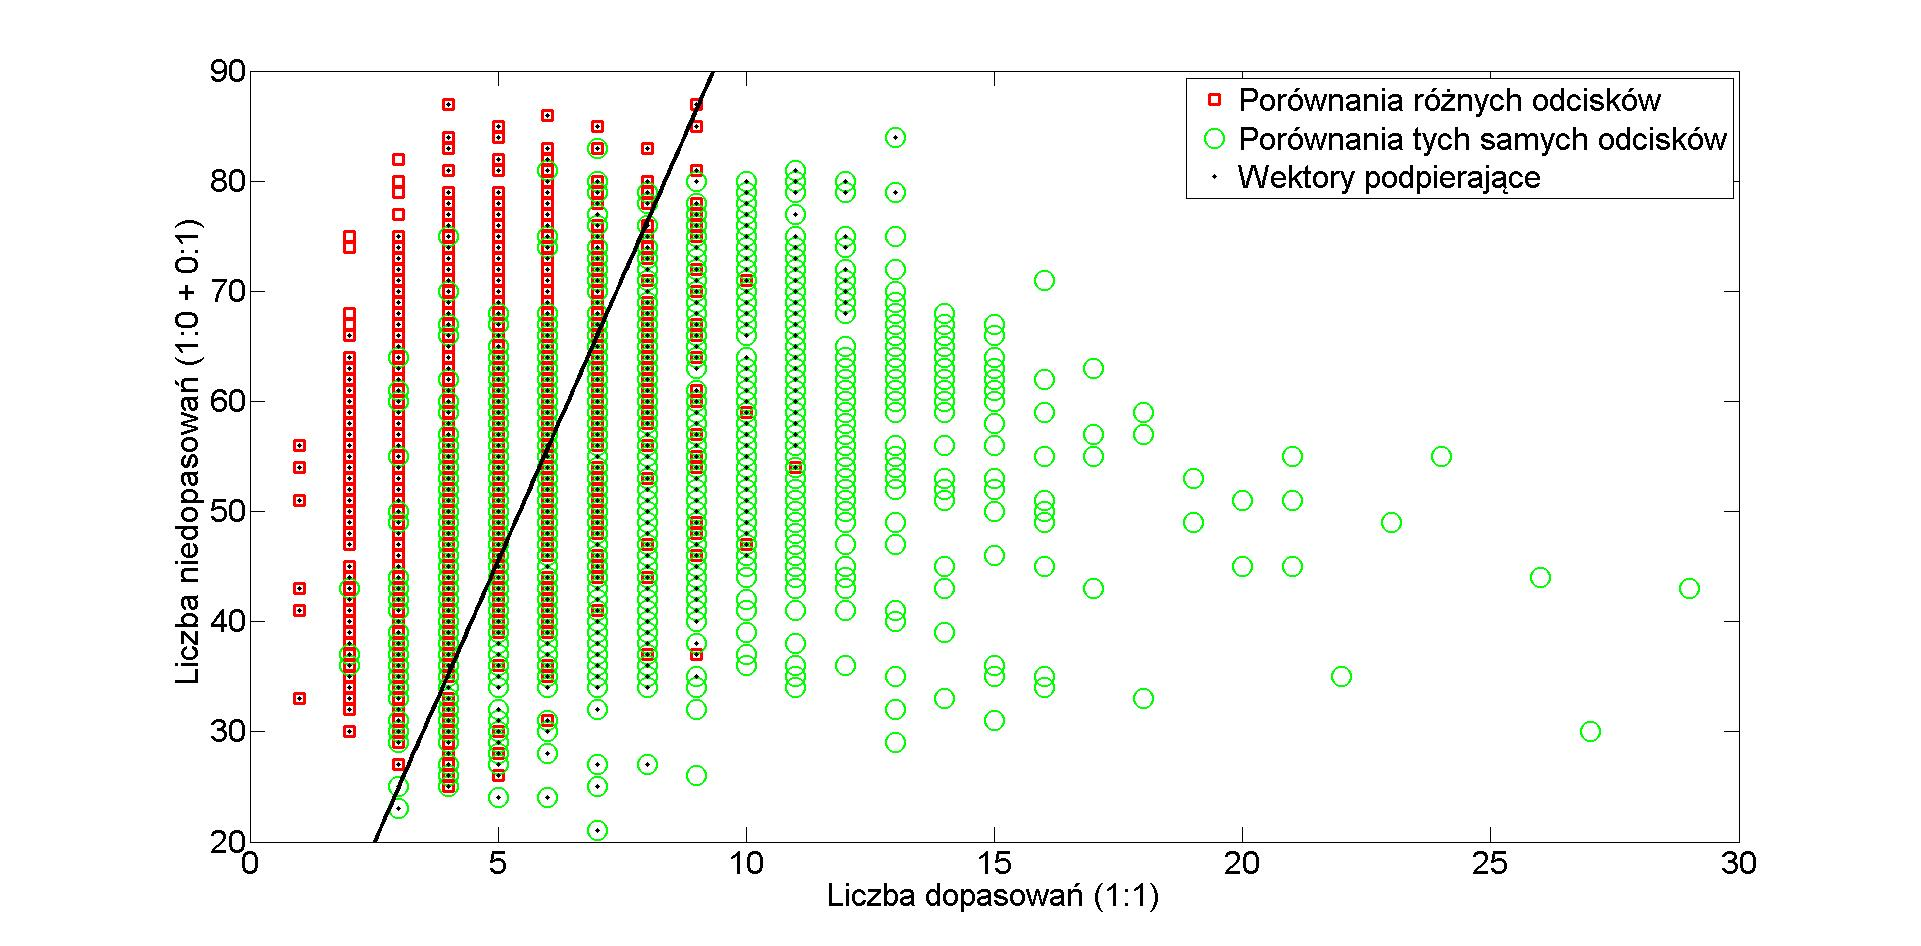
\includegraphics[angle=0,scale=0.27]{img/SVM_linear_code_1.jpg}
		\caption{Separacja punktów dla jądra liniowego}
		\label{img:SVM_linear_code_1}
    \end{center}
\end{figure} 

Wykres \ref{img:SVM_linear_code_1} przedstawia liniową separacje punktów. Konsekwentnie zielonym kolorem zaznaczone są porównania między odciskami pochodzącymi od tego samego palca, czerwonym porównania między odciskami pochodzącymi od różnych palców. Doskonale widać iż nie możliwe jest liniowe separowanie punktów. Metoda już dla zbioru testowego wniesie pewien błąd. Nie jest to jednak ogromny problem. Możliwe jest bowiem stworzenie kilku równań prostych które w stu procentach rozdzielą oba zbiory. Niestety nie wpływa to na skuteczność metody, zbiór uczący powinien być w miarę uniwersalny, a funkcja powinna tylko uogólniać zachowanie punktów na płaszczyźnie. 

    \begin{table}[!htb]
    \begin{tabular}{p{3cm}|r||c|c|c|}
	\cline{2-5}
    & Wariant & \multicolumn{3}{|c|}{1:1 do 1:0 + 0:1}\\ \cline{2-5} 
    & Zbiór testujący & ERRORS  & FRR & FAR\\ \hline
	\multicolumn{2}{|l||}{Rodzaj jądra} &  \multicolumn{3}{|c|}{}\\
	\hline\hline
    \multicolumn{2}{|l||}{Liniowe} & 28.6722\% & 26.6393\% & 31.405\%\\ \hline
    \multicolumn{2}{|l||}{Kwadratowe} & 28.6722\% & 25.6148\% & 32.7824\%\\ \hline
    \multicolumn{2}{|l||}{Wielomianowe st. 3} & 28.9072\% & 29.3033\% & 28.3747\%\\ \hline
    \multicolumn{2}{|l||}{Wielomianowe st. 7} & 31.2573\% & 29.3033\% & 33.8843\%\\ \hline
    \multicolumn{2}{|l||}{Wielomianowe st. 12} & 29.3772\% & 32.7869\% & 24.7934\%\\ \hline
    \multicolumn{2}{|l||}{Normalne(Gaussowskie)} & 28.6722\% & 24.7951\% & 33.8843\%\\ \hline
    \end{tabular}
	\caption{Wyniki testów algorytmu kodowego metoda 3D porównywania kodów}
	\label{tab:3D_sum}
    \end{table}
    
    \begin{table}[!htb]
    \begin{tabular}{p{3cm}|r||c|c|c|}
	\cline{2-5}
    & Wariant & \multicolumn{3}{|c|}{1:1 do 1:0} \\ \cline{2-5} 
    & Zbiór testujący & ERRORS  & FRR & FAR\\ \hline
	\multicolumn{2}{|l||}{Rodzaj jądra} &  \multicolumn{3}{|c|}{}\\
	\hline\hline
    \multicolumn{2}{|l||}{Liniowe} & 29.6703\% & 13.6232\% & 57.2139\%\\ \hline
    \multicolumn{2}{|l||}{Kwadratowe} & 29.8535\% & 12.4638\% & 59.7015\%\\ \hline
    \multicolumn{2}{|l||}{Wielomianowe st. 3} & 29.3040\% & 7.8261\% & 66.1692\%\\ \hline
    \multicolumn{2}{|l||}{Wielomianowe st. 7} & 30.2198\% & 8.9855\% & 66.6667\%\\ \hline
    \multicolumn{2}{|l||}{Wielomianowe st. 12} & 36.8132\% & 35.3623\% & 39.3035\%\\ \hline
    \multicolumn{2}{|l||}{Normalne(Gaussowskie)} & 31.1355\% & 3.7681\% & 78.1095\%\\ \hline
    \end{tabular}
	\caption{Wyniki testów algorytmu kodowego metoda 3D porównywania kodów}
	\label{tab:3D_pattern}
    \end{table}
    
    \begin{table}[!htb]
    \begin{tabular}{p{3cm}|r||c|c|c|}
	\cline{2-5}
    & Wariant & \multicolumn{3}{|c|}{1:1 do 0:1} \\ \cline{2-5} 
    & Zbiór testujący & ERRORS  & FRR & FAR\\ \hline
	\multicolumn{2}{|l||}{Rodzaj jądra} &  \multicolumn{3}{|c|}{}\\
	\hline\hline
    \multicolumn{2}{|l||}{Liniowe} & 31.2024\% & 30.2778\% & 32.3232\% \\ \hline
    \multicolumn{2}{|l||}{Kwadratowe} & 30.5936\% & 31.6667\% & 29.2929\%\\ \hline
    \multicolumn{2}{|l||}{Wielomianowe st. 3} & 31.3546\% & 29.7222\% & 33.3333\%\\ \hline
    \multicolumn{2}{|l||}{Wielomianowe st. 7} & 34.2466\% & 43.0556\% & 23.5690\%\\ \hline
    \multicolumn{2}{|l||}{Wielomianowe st. 12} & 32.5723\% & 36.3889\% & 27.9461\%\\ \hline
    \multicolumn{2}{|l||}{Normalne(Gaussowskie)} & 31.2024\% & 29.7222\% & 32.9966\%\\ \hline
    \end{tabular}
	\caption{Wyniki testów algorytmu kodowego metoda 3D porównywania kodów}
	\label{tab:3D_sample}	
    \end{table}
    
   \begin{figure}[!htb]
    \begin{center}
		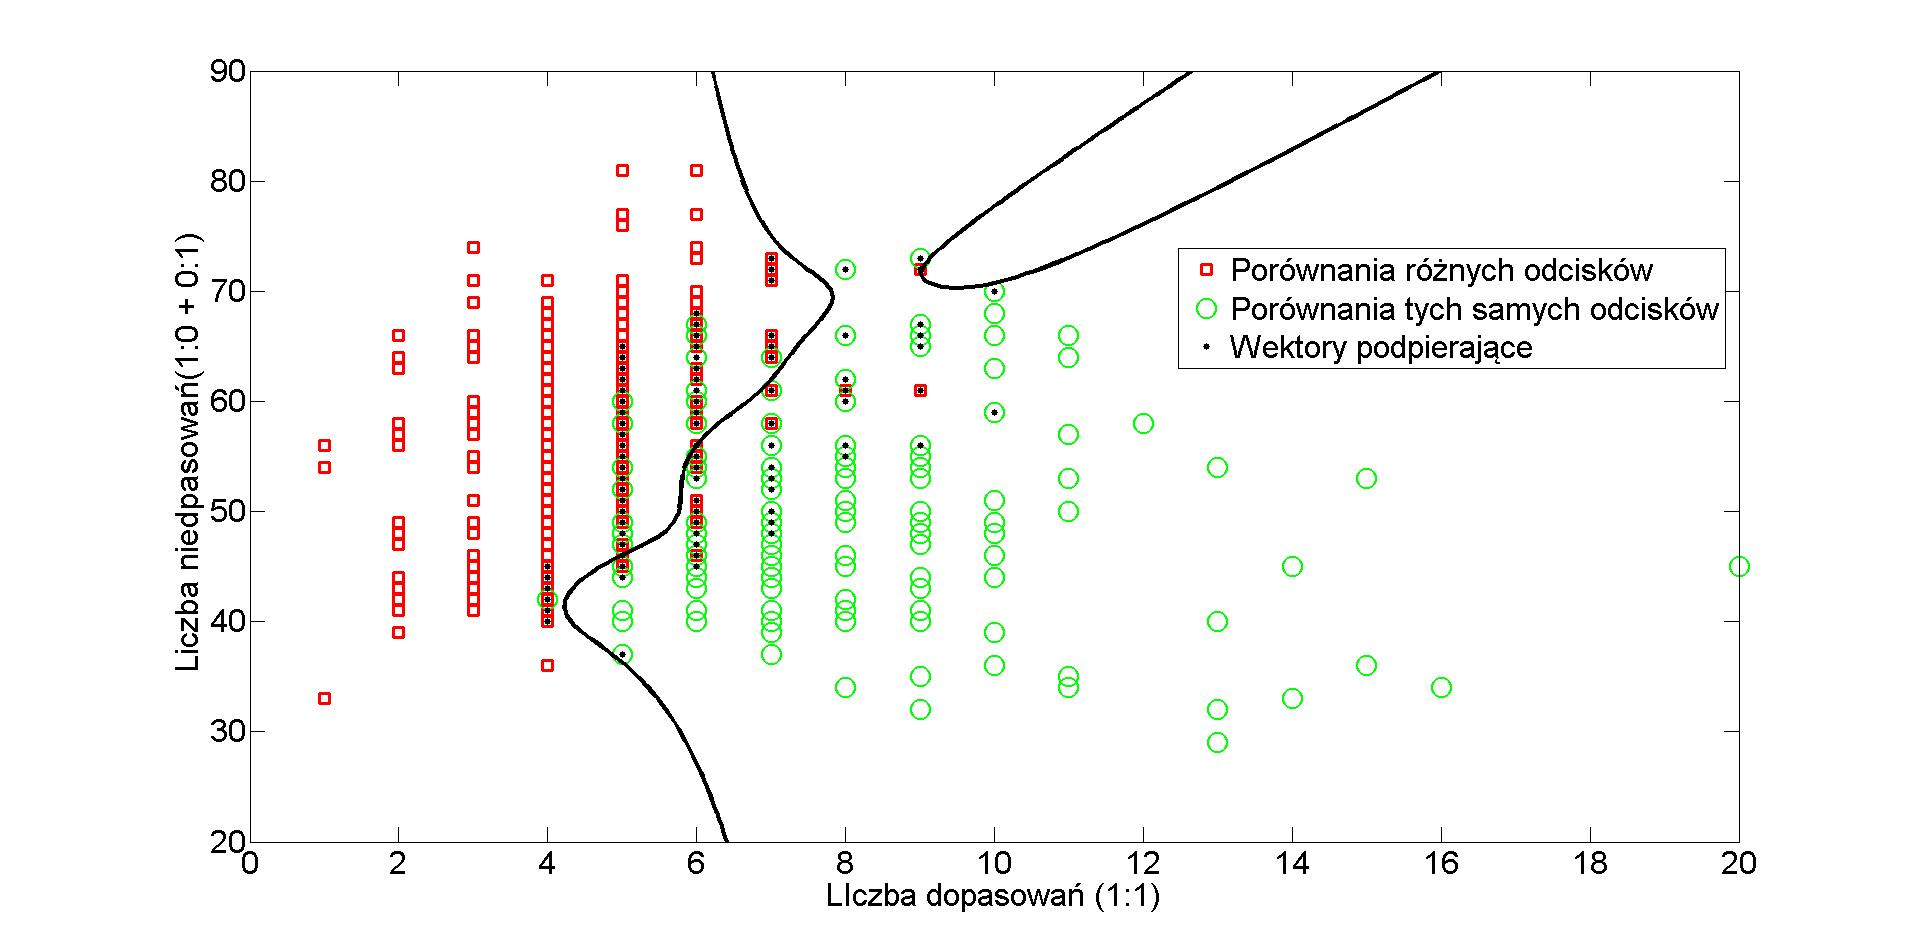
\includegraphics[angle=0,scale=0.27]{img/SVM_polynominal_code_1.jpg}
		\caption{Separacja punktów dla jądra wielomianowego stopnia 7}
		\label{img:SVM_polynominal_code_1}
    \end{center}
    \end{figure}
    
    \begin{figure}[!htb]
    \begin{center}
		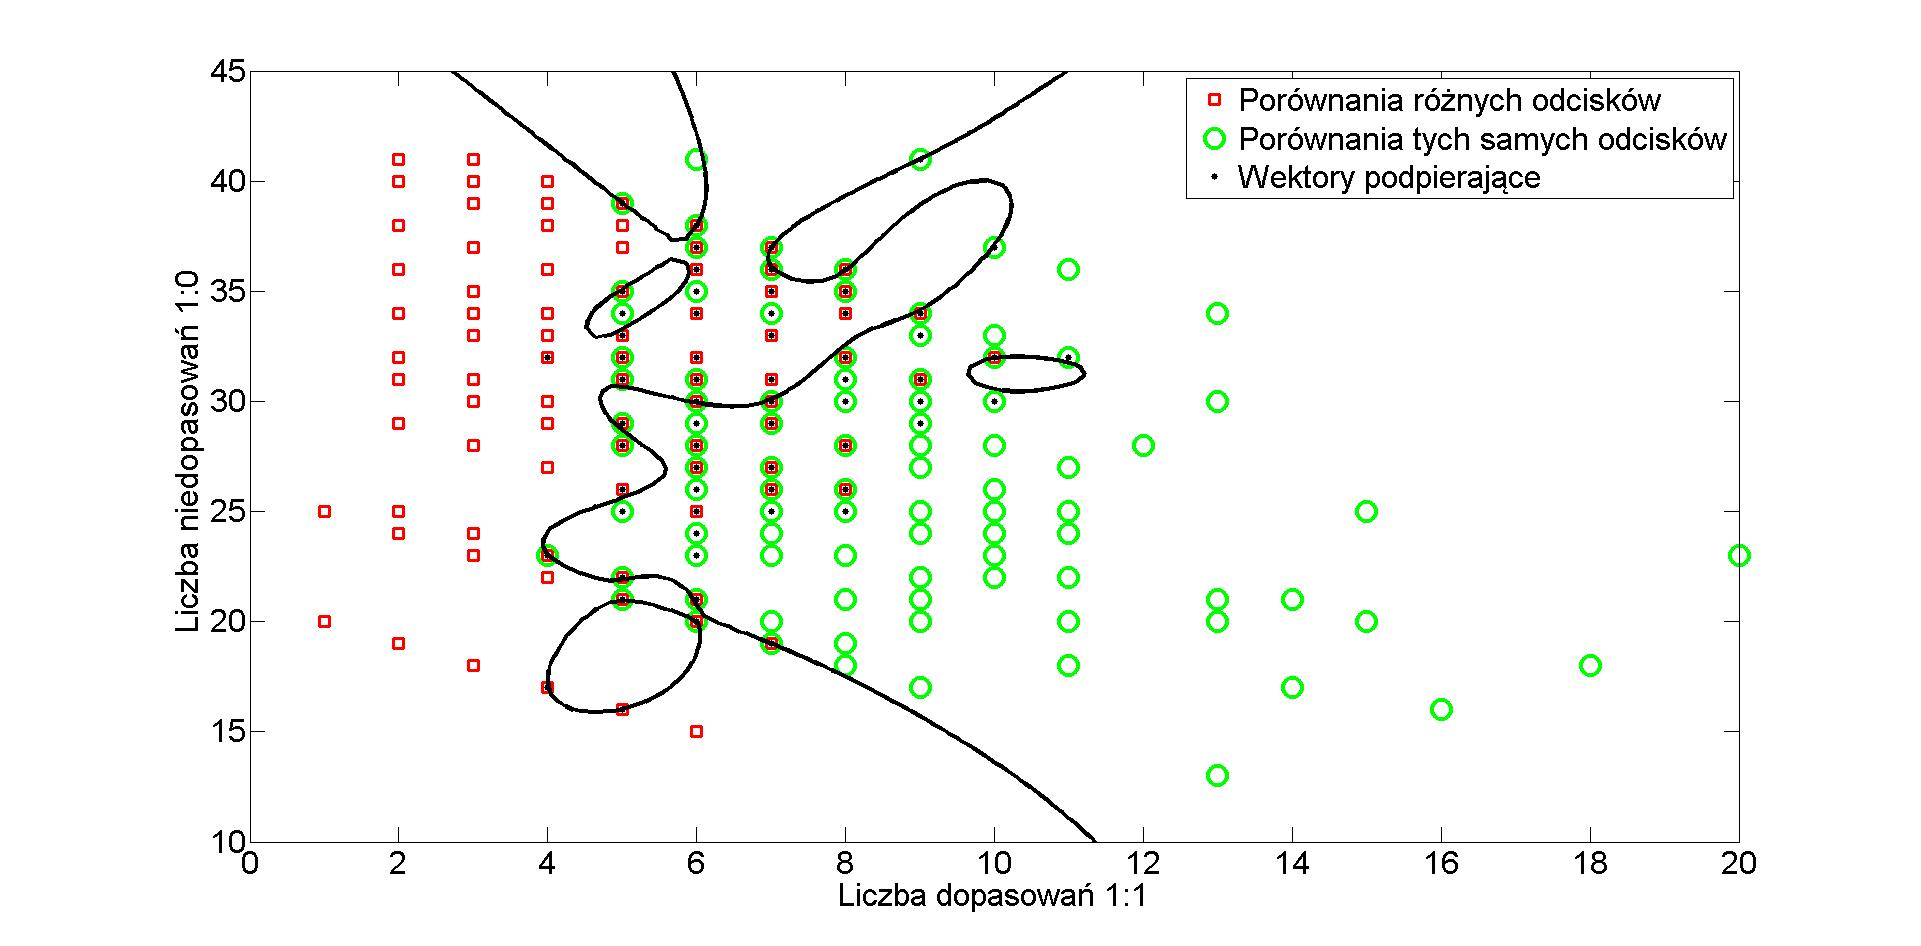
\includegraphics[angle=0,scale=0.27]{img/bad_st_12.jpg}
		\caption{Zły wpływ zbyt dużego stopnia jądra wielomianowego(12)}
		\label{img:best_SVM}
    \end{center}
    \end{figure} 
    
    \begin{figure}
    \begin{center}
		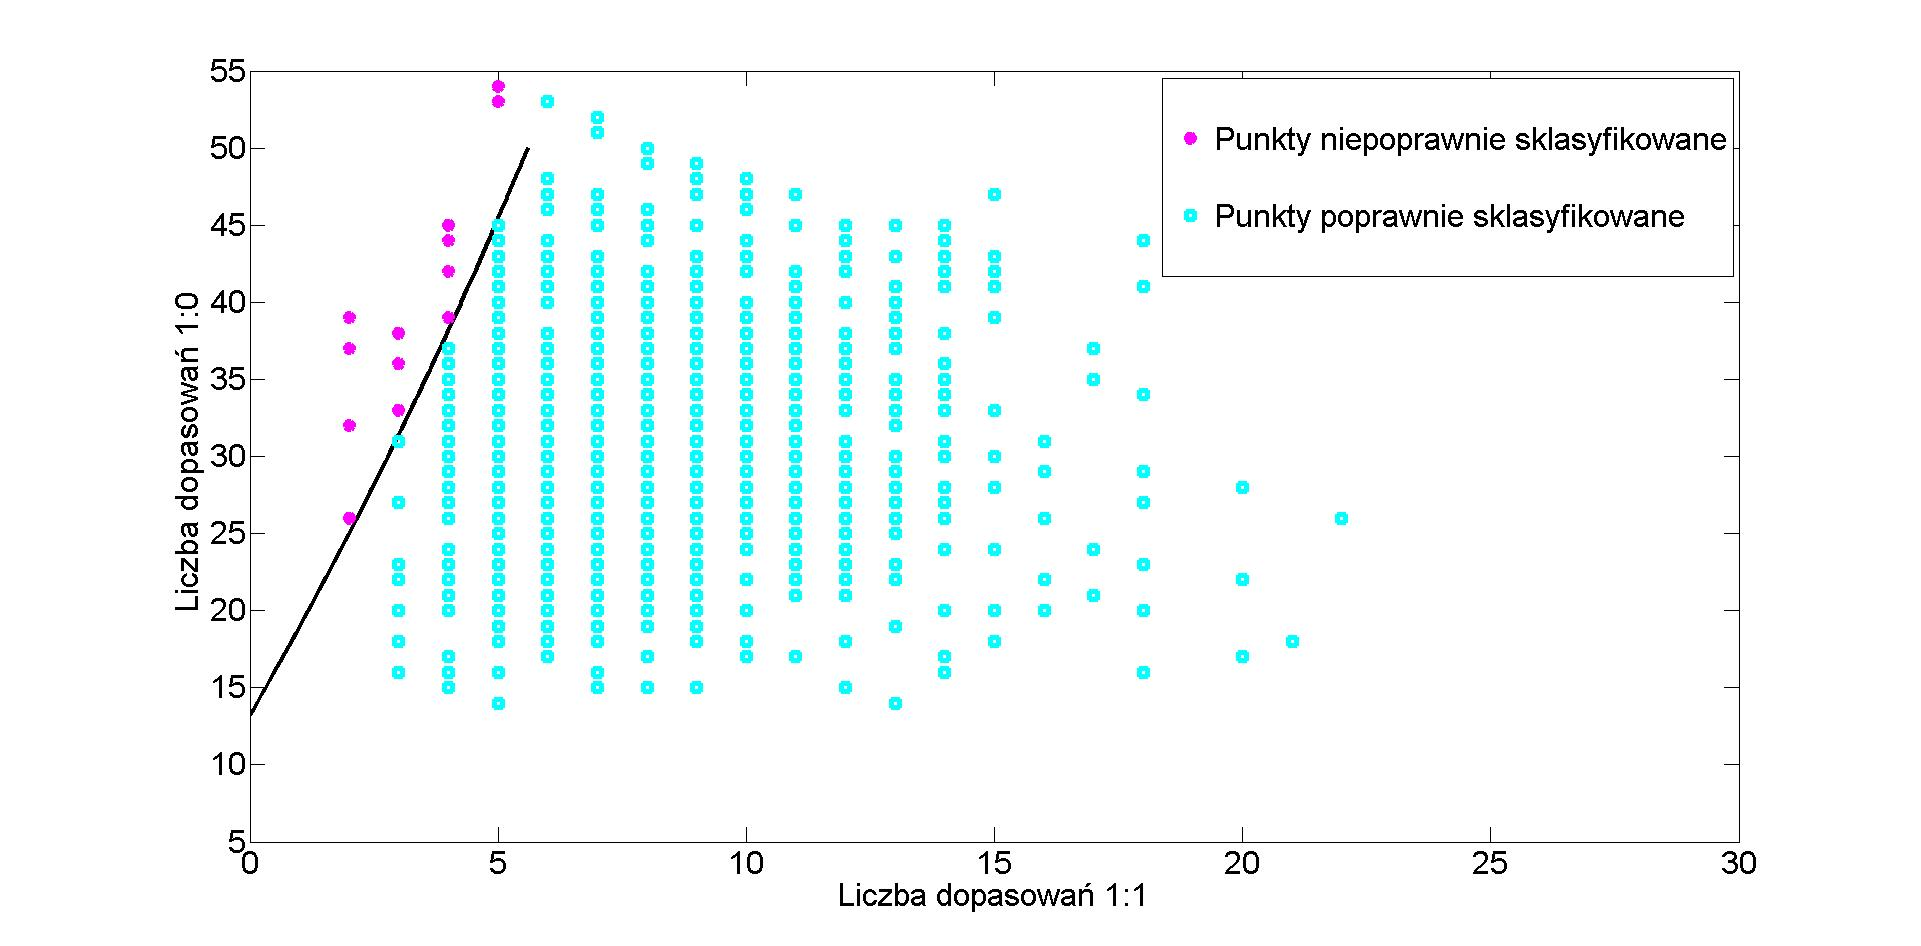
\includegraphics[angle=0,scale=0.27]{img/3D_best_score.jpg}
		\caption{Przykład klasyfikacji punktów algorytmu kodującego dla wariantu 1:1 do 1:0 jądro gaussowskie}
		\label{img:bad_SVM}
    \end{center}
    \end{figure} 
    
Tabele \ref{tab:3D_sum}, \ref{tab:3D_pattern}, \ref{tab:3D_sample} przedstawiają wyniki dla algorytmu kodującego. Widać, że pierwotne przypuszczenia rokujące poprawę jakości dopasowania były błędne. wyniki porównań znacznie się pogorszyły. Może to wynikać z niemożności znalezienia krzywej która w pełni separuje grupy punktów. Dodatkowo żaden z wariantów porównywania nie wyróżnia się na tle innych. Ilość błędnych decyzji jest podobna dla wszystkich wariantów i waha się od 28\% do 35\%. Jedyną wyraźną poprawę widać dla wskaźnika FRR dla wariantu porównań 1:1 do 1:0, gdzie dla jądra gaussowskiego wskaźnik ten wynosi ok 3\% , gdzie dla poprzednich metod wahał się od 17\% do 23\%. Niestety FAR dla tej metody wynosi ponad 78\% co oznacza iż skuteczniejszy byłby tu klasyfikator losowy. Poprawę wskaźnika FRR można motywować tym iż klasyfikator SVM uczył się tylko na wynikach wzorca, gdyż oba porównania 1:1 i 1:0 dotyczą minucji wzorca. Niestety analogiczna sytuacja dla próbki gdzie klasyfikator uczył się na porównaniach 1:1 i 0:1 nie wykazała poprawy dla wskaźnika FAR. Gdyby tak się stało sensowne było by uczenie się na klasyfikatora SVM nie w przestrzenie dwu a trzy-wymiarowej. Dodatkowo większe skomplikowanie funkcji separującej nie przyczynia się do wzrostu tylko do spadku jakości porównania. Ponieważ nie do się idealnie rozsmarować punktów najlepiej spisują się metody o liniowym kształcie hiperprzestrzeni metody SVM. Zbyt zawiła funkcja prowadzi do bezsensownych rozgraniczeń takich ja pokazanych na rysunku \ref{img:bad_SVM}.

\begin{table}[!htb]
    \begin{tabular}{p{3cm}|r||c|c|c|}
	\cline{2-5}
    & Wariant & \multicolumn{3}{|c|}{1:1 do 1:0 + 0:1}\\ \cline{2-5} 
    & Zbiór testujący & ERRORS  & FRR & FAR\\ \hline
	\multicolumn{2}{|l||}{Rodzaj jądra} &  \multicolumn{3}{|c|}{}\\
	\hline\hline
    \multicolumn{2}{|l||}{Liniowe} & 0.4975\% & 0.0\% & 1.3889\%\\ \hline
    \multicolumn{2}{|l||}{Kwadratowe} & 0.4975\% & 0.0\% & 1.3889\%\\ \hline
    \multicolumn{2}{|l||}{Wielomianowe st. 3} &0.4975\% & 0\% & 1.3889\%\\ \hline
    \multicolumn{2}{|l||}{Wielomianowe st. 7} & 0.9950\% & 0.7752\% & 1.3889\%\\ \hline
    \multicolumn{2}{|l||}{Wielomianowe st. 12} & 0.9950\% & 0.7752\% & 1.3889\%\\ \hline
    \multicolumn{2}{|l||}{Normalne(Gaussowskie)} & 0.4975\% & 0\% & 1.3889\%\\ \hline
    \end{tabular}
	\caption{Wyniki testów algorytmu kodowego metoda 3D porównywania kodów}
	\label{tab:3D_sum_2}
    \end{table}
    
    \begin{table}[!htb]
    \begin{tabular}{p{3cm}|r||c|c|c|}
	\cline{2-5}
    & Wariant & \multicolumn{3}{|c|}{1:1 do 1:0} \\ \cline{2-5} 
    & Zbiór testujący & ERRORS  & FRR & FAR\\ \hline
	\multicolumn{2}{|l||}{Rodzaj jądra} &  \multicolumn{3}{|c|}{}\\
	\hline\hline
    \multicolumn{2}{|l||}{Liniowe} & 2.5641\% & 2.0\% & 5.8824\%\\ \hline
    \multicolumn{2}{|l||}{Kwadratowe} & 1.7094\% & 1.0\% & 5.8824\%\\ \hline
    \multicolumn{2}{|l||}{Wielomianowe st. 3} & 1.7094\% & 1.0\% & 5.8824\%\%\\ \hline
    \multicolumn{2}{|l||}{Wielomianowe st. 7} & 2.5641\% & 2.0\% & 5.8824\%\\ \hline
    \multicolumn{2}{|l||}{Wielomianowe st. 12} & 6.8376\% & 7.0\% & 5.8824\%\\ \hline
    \multicolumn{2}{|l||}{Normalne(Gaussowskie)} & 11.1111\% & 0\% & 76.4706\%\\ \hline
    \end{tabular}
	\caption{Wyniki testów algorytmu kodowego metoda 3D porównywania kodów}
	\label{tab:3D_pattern}
    \end{table}
    
    \begin{table}[!htb]
    \begin{tabular}{p{3cm}|r||c|c|c|}
	\cline{2-5}
    & Wariant & \multicolumn{3}{|c|}{1:1 do 0:1} \\ \cline{2-5} 
    & Zbiór testujący & ERRORS  & FRR & FAR\\ \hline
	\multicolumn{2}{|l||}{Rodzaj jądra} &  \multicolumn{3}{|c|}{}\\
	\hline\hline
    \multicolumn{2}{|l||}{Liniowe} & 1.0638\% & 0.9091\% & 1.2821\% \\ \hline
    \multicolumn{2}{|l||}{Kwadratowe} & 0.5319\% & 0.0\% & 1.2821\%\\ \hline
    \multicolumn{2}{|l||}{Wielomianowe st. 3} & 0.5319\% & 0.0\% & 1.2821\%\\ \hline
    \multicolumn{2}{|l||}{Wielomianowe st. 7} & 1.0638\% & 0.9091\% & 1.2821\%\\ \hline
    \multicolumn{2}{|l||}{Wielomianowe st. 12} & 1.5957\% & 1.8182\% & 1.2821\%\\ \hline
    \multicolumn{2}{|l||}{Normalne(Gaussowskie)} & 0.5319\% & 0.0\% & 1.2821\%\\ \hline
    \end{tabular}
	\caption{Wyniki testów algorytmu kodowego metoda 3D porównywania kodów}
	\label{tab:3D_sample}	
    \end{table}
    
    Dla SDK $Neurotechnology$ wyniki generalnie uległy poprawie wahając się pierwotnie w granicach 0.8\% - 1.5\% dla porównywania oddzielnie podobieństwa i niepodobieństwa do najlepszych wyników ok 0.5\% dla porównywania 3D. Dla SDK najkorzystniejszym wariantem okazał się wariant uwzględniający porównania 1:1 do sumy 1:0 i 0:1. Przyczyną poprawy jest możliwość znalezienia funkcji "niemalże" separujących grupy punktów. Oznacza to, że sposób porównywania podobieństwa i niepodobieństwa jednocześnie podnosi skuteczność porównań. warunkiem koniecznym takiego zachowania jest możliwość separowania punktów porównań. W przeciwnym wypadku metoda prowadzi do pogarszania wyników.
    
\section[Wnioski][Wnioski]{Wnioski}

Metoda 3D porównywania kodów jest metodą której skuteczność jest ściśle uzależniona od rozkładu punktów  na płaszczyźnie i możliwości ich oddzielenia od siebie. W przypadku punktów których nie można odseparować metoda jedynie pogorszy uzyskiwane wyniki w stosunku do porównań tylko jednej cechy. Nie wskazane jest używanie zbyt zawiłych funkcji separujących. Klasyfikator powinien jedynie określać przybliżony rozkład punktów funkcje złożone powodują uczenie się na podstawie pojedynczych punktów, które nie mają odzwierciedlenia do całości zbioru porównań odcisków. Metoda nie gwarantuje 100\% skuteczności porównywania odcisków, ale istnieją takie konfiguracje metody gdzie pojedyncze współczynniki są pozbawione błędu(np FRR dla jadra liniowego wariantu porównań 1:1 do sumy 1:0 i 0:1 dla SDK $Neurotechnology$). Nie należy się jednak sugerować zbytnio otrzymanymi wynikami, twierdząc że powstała metoda bezbłędnie klasyfikująca odciski. Wszystko zależy od zbiory uczącego i zbioru testującego. 
Jednak opisana tu metoda dla SDK $Neurotechnology$ jest najlepszą z przedstawianych metod. 
 
    